\afterpage{%
	\clearpage
	
	\begin{landscape}
	
		\begin{figure*}[p]
			\centering
			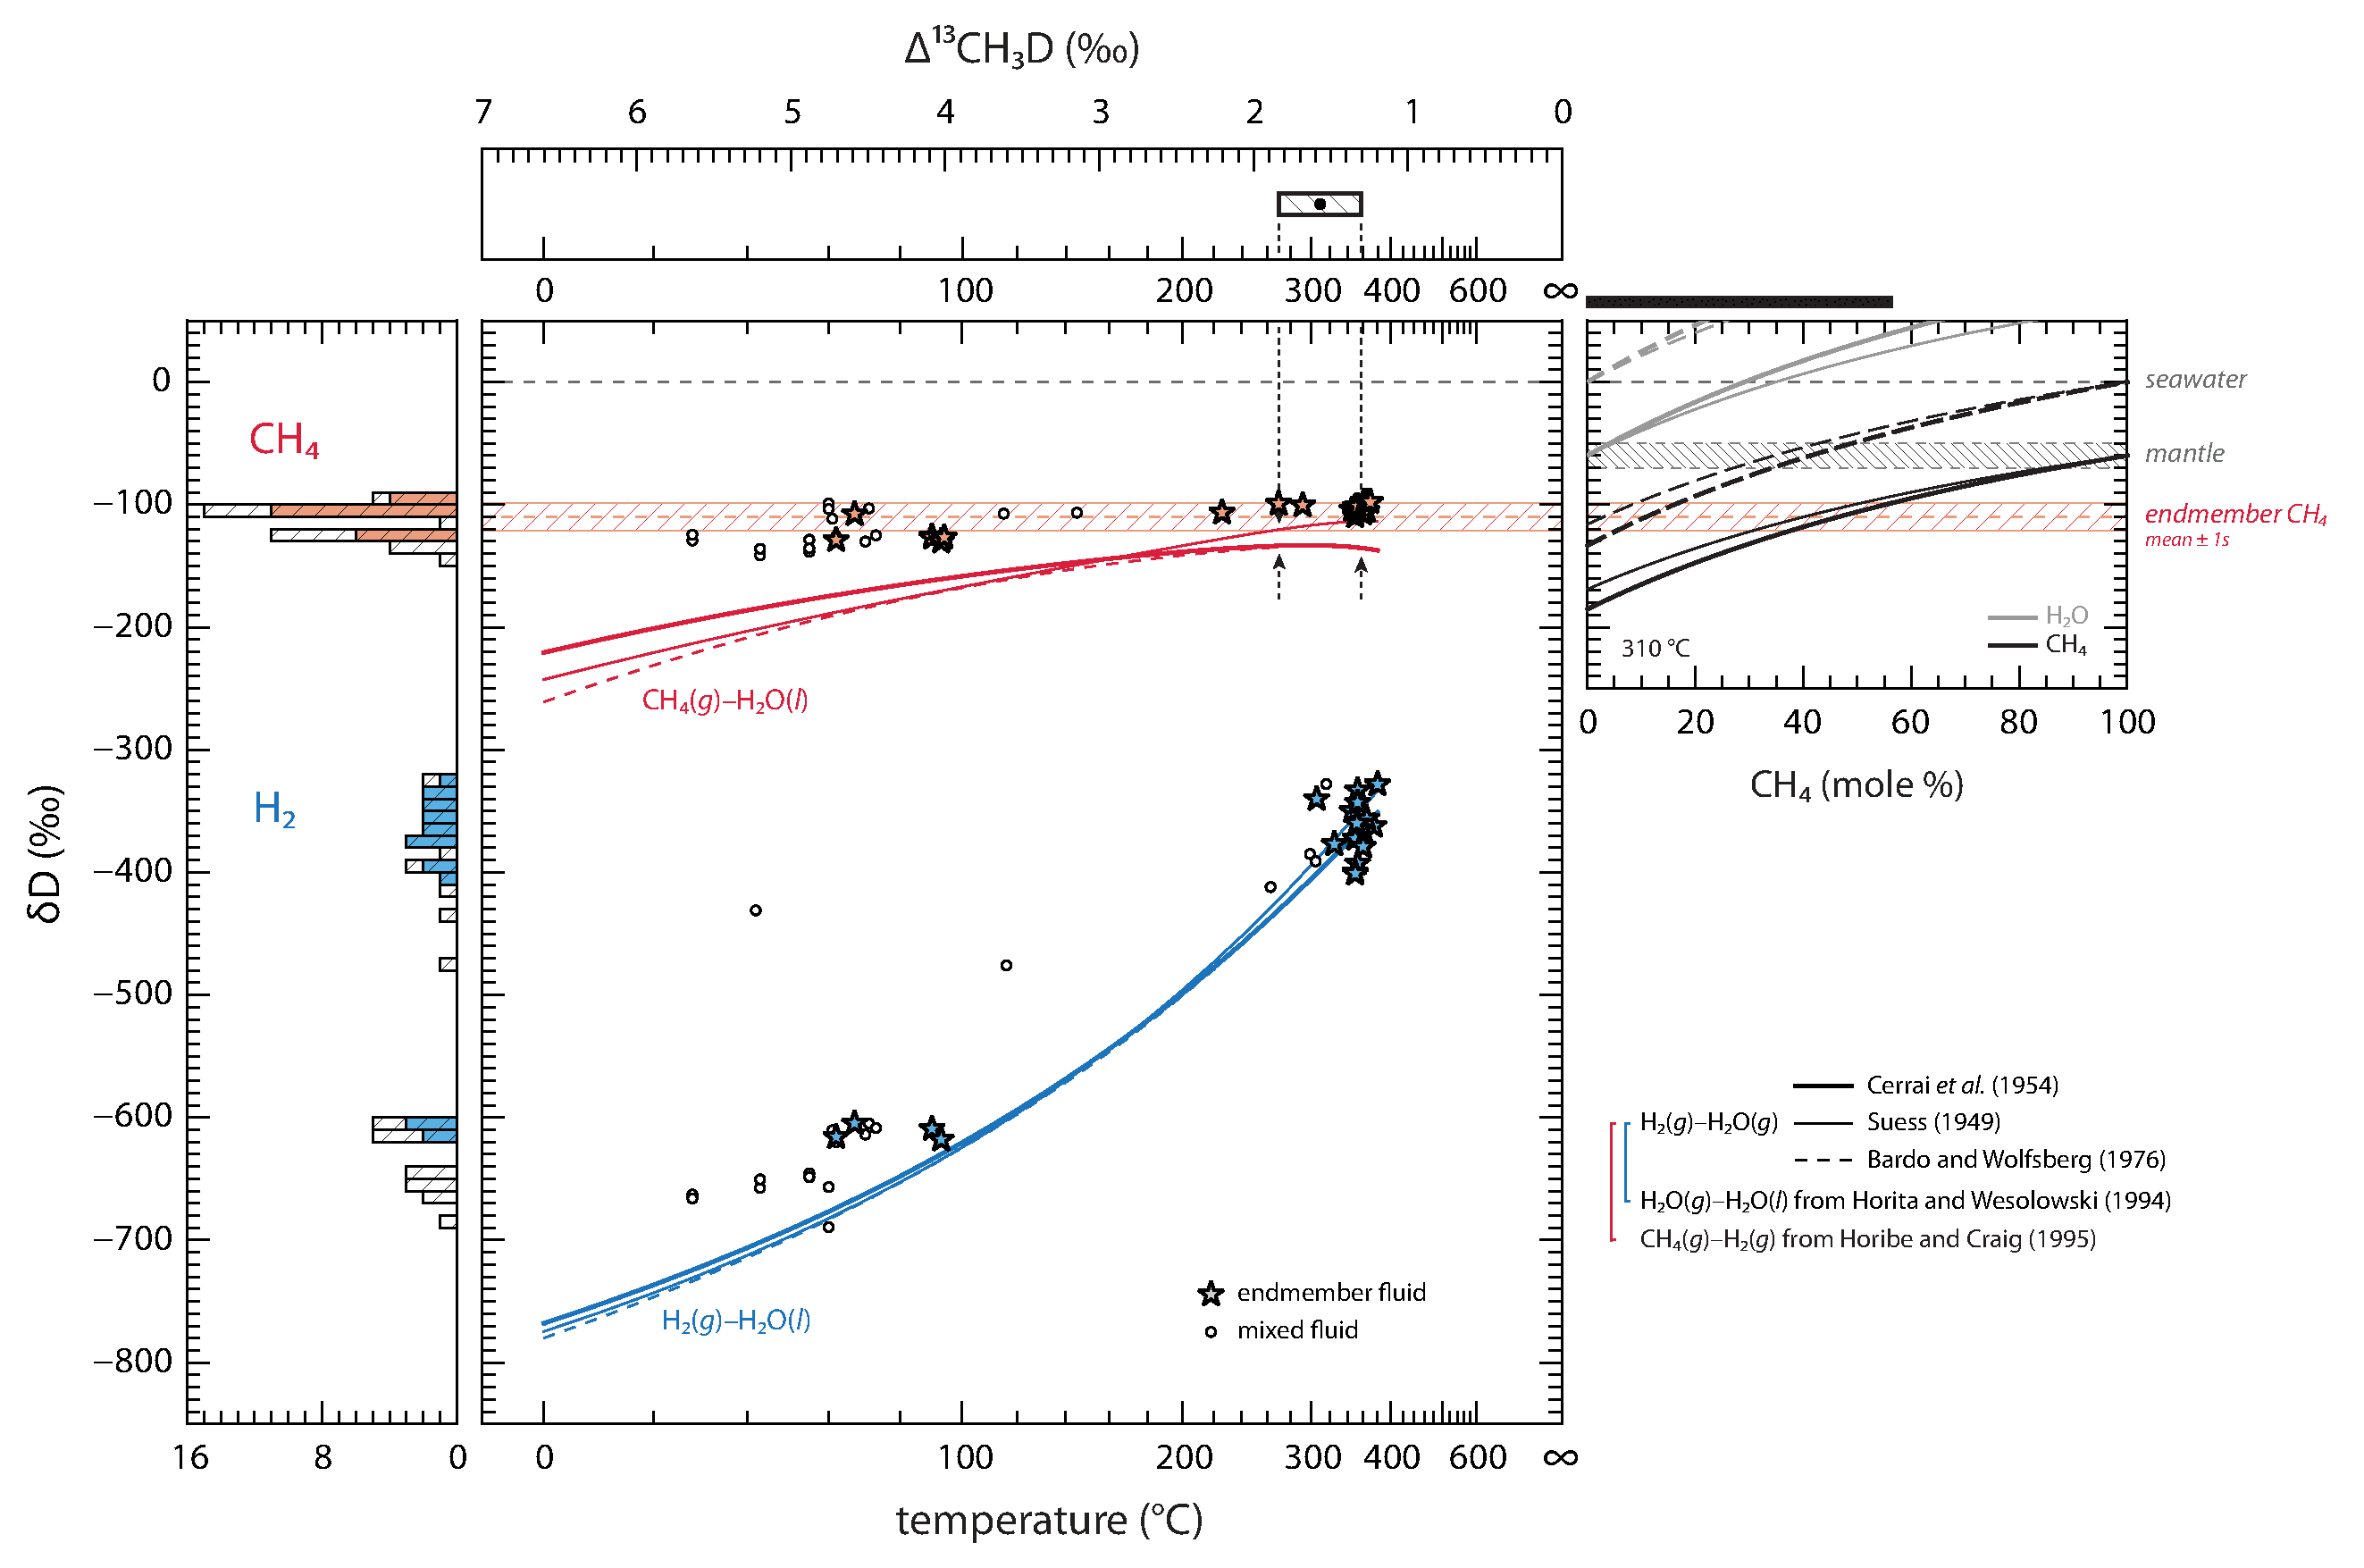
\includegraphics[width=\linewidth]{figures/Fig3.5}
			
			
			
		\end{figure*}
	
	\end{landscape}
	%\addtocounter{figure*}{-1}	% decrement counter because putting figure caption in next float
	
	\begin{landscape}
		
		\begin{figure*}[h!]
			\caption[Data and models of D/H of CH\textsubscript{4} and H\textsubscript{2} in seafloor hydrothermal fluids]{%
			Hydrogen
			isotopic composition of CH\textsubscript{4} (red) and H\textsubscript{2}
			(blue) in seafloor hydrothermal fluids plotted against measured vent
			temperatures. Data are from unsedimented fields studied in \textcite{Welhan+Craig_1983,Proskurowski++_2006_CG,Kawagucci++_2010_JGR,Charlou++_2010}, and in this study (see \mrefs[]{Tables}{tab:3:1} and~\ref{tab:3:1}), and are tabulated in
			\autoref{tab:3:S1}. Endmember fluids (identified by low Mg contents)
			are represented by stars, and vent fluids containing a mixture of
			hydrothermal endmember fluid and seawater are represented by circles.
			Data from sites exhibiting phase separation \parencite{Charlou++_2010} or
			with fluids diffusely effluxing through colonies of deep-sea snails or
			shrimp \parencite{Kawagucci++_2010_JGR} are excluded from this plot (see notes
			under \autoref{tab:3:S1}). Red hatching indicates the average δD of
			CH\textsubscript{4} in endmember fluids ($-$110 ± 12‰, 1\emph{s}) in the
			compiled dataset. Red and blue curves represent the δD values of
			CH\textsubscript{4} and H\textsubscript{2} (respectively) in D/H
			equilibrium with H\textsubscript{2}O of seawater-like isotopic
			composition (δD = 0‰, dashed gray line) predicted by combinations of
			published calibrations for
			H\textsubscript{2}(\emph{g})/H\textsubscript{2}O(\emph{g}) \parencite{Suess_1949,Cerrai++_1954,Bardo+Wolfsberg_1976_JPC},
			H\textsubscript{2}O(\emph{g})/H\textsubscript{2}O(\emph{l}) \parencite{Horita+Wesolowski_1994_GCA}, and
			CH\textsubscript{4}(\emph{g})/H\textsubscript{2}(\emph{g}) \parencite{Horibe+Craig_1995_GCA}. {[}High-temperature hydrothermal fluids generally have δD
			values of H\textsubscript{2}O close to 0‰ \parencite{Shanks++_1995_AGU-GM}. Note
			that measured values for δD of H\textsubscript{2}O in fluids from Lost
			City are +2 to +7‰ \parencite{Proskurowski++_2006_CG} and thus the equilibrium
			values for CH\textsubscript{4} and H\textsubscript{2} at Lost City are
			slightly (\textasciitilde{}5‰) higher than those indicated by the
			curves; this difference is small compared to the uncertainty in
			equilibrium fractionation factor calibrations at the temperatures of
			these fluids (\textasciitilde{}30 to 90~°C).{]} (\emph{\textbf{Left}})
			Histogram of δD values of CH\textsubscript{4} and H\textsubscript{2} in
			endmember (shaded) and mixed fluids (unshaded bars).
			(\emph{\textbf{Top}}) Mean ± 1\emph{s} of the
			Δ\textsuperscript{13}CH\textsubscript{3}D values and corresponding
			clumped isotopologue temperatures (\(310_{- 42}^{+ 53}\)~°C) of methane
			reported in \autoref{tab:3:1}. Dashed black arrows point to the range of δD values
			of CH\textsubscript{4}(\emph{g}) in equilibrium with seawater at the
			temperatures indicated by Δ\textsuperscript{13}CH\textsubscript{3}D
			data. (\emph{\textbf{Right}}) Modeled δD values of CH\textsubscript{4}
			(black curves) and H\textsubscript{2}O (gray curves) as a function of
			mole fraction of CH\textsubscript{4} in a hypothetical methane-rich
			fluid. All H was assumed to exist as H\textsubscript{2}O(\emph{l}) in
			isotopic equilibrium with CH\textsubscript{4}(\emph{g}) at the
			temperature indicated by the mean
			Δ\textsuperscript{13}CH\textsubscript{3}D value (310~°C). {[}At
			\textasciitilde{}270 to 360~°C, D/H fractionation between
			CH\textsubscript{4}(\emph{g}) and H\textsubscript{2}O(\emph{l}) is not
			very sensitive to temperature \parencite{Horibe+Craig_1995_GCA}. Uncertainty in
			the equilibrium D/H fractionation factor is dominated by the
			disagreement among
			H\textsubscript{2}(\emph{g})/H\textsubscript{2}O(\emph{g}) calibrations.
			Isotopic fractionation between CH\textsubscript{4}(\emph{g}) and
			CH\textsubscript{4}(\emph{aq}) is negligible \parencite{Bacsik++_2002_JCP}, and
			the fractionation between H\textsubscript{2}O(\emph{g}) and
			H\textsubscript{2}O(\emph{l}) is small (\textasciitilde{}5‰) \parencite{Horita+Wesolowski_1994_GCA}. The model neglects the effects of elevated pressure
			and salinity \parencite{Horita_2005_GcJ,Martineau++_2012_CG}, and ignores
			potential isotopic exchange with hydrous minerals \parencite{Horita++_1999_S,Saccocia++_2009_GCA,Meheut++_2010_GCA}.{]} The initial δD was taken
			to be 0‰ (dashed lines) for seawater-derived H, or $-$60‰ (solid lines)
			for mantle-derived H \parencite{Clog++_2013_EPSL}. Minimum and maximum values
			expected for δD of CH\textsubscript{4} are represented by the solid and
			dashed lines, respectively. Mixing of seawater with mantle-derived water
			prior to respeciation of H\textsubscript{2}O to CH\textsubscript{4} and
			re-equilibration of CH\textsubscript{4} initially formed in equilibrium
			with mantle-derived H\textsubscript{2}O (both resulting in δD values of
			CH\textsubscript{4} moving upwards towards the dashed lines) affect the
			predictions; effects of these processes are treated in \autoref{sec:3:discussion}. The black bar shows the range in CH\textsubscript{4}
			mole fraction that is compatible with the isotopic data from vent
			fluids.
		}
		\label{fig:3:5}
	\end{figure*}
	
	\clearpage
}

\end{landscape}